% !TeX spellcheck = en_US
\documentclass[]{scrartcl}

\usepackage{graphicx}
\usepackage{graphics}
\usepackage{hyperref}

%opening
\title{}
\author{}

\begin{document}

\maketitle

\begin{abstract}

\end{abstract}

\section{Romanza}

\subsection{4.a) Original sound signal}\label{sec:4}
The digital sound signal stored in file {\texttt romanza\textunderscore pe.wav}, that was provided, was uploaded to MATLAB. It corresponds to the digitization of an original analog sound signal with a sampling rate of $f_s = 44.1$kHz.

The digital signal plays a sharp melody of a violin playing. To analyze the digital sound signal in the frequency domain, its spectrogram was plotted. It is presented, for the first 15s of the signal, in Fig. \ref{fig:spctOriginal}, with a window of $N = 2400$. Whenever a certain note is played on the violin, the cords vibrate at a specific combination of harmonics, which are integer multiples of a fundamental frequency. In fact, these harmonics are noticeable in the spectrogram of Fig. \ref{fig:spctOriginal}.

\begin{figure}[htbp]
	\centering
	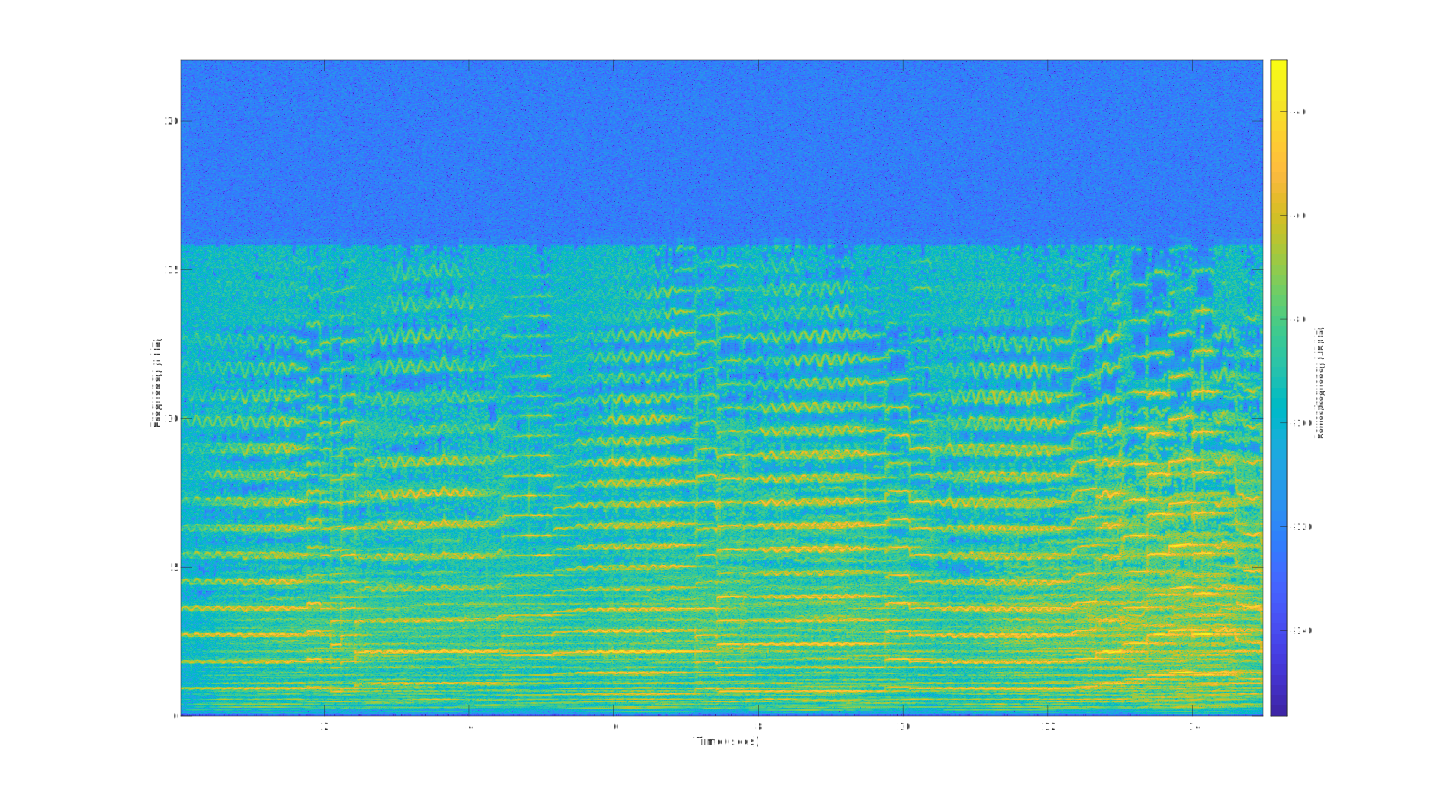
\includegraphics[width=1\textwidth]{figures/spect_original.png}
	\caption{Spectrogram of the original digital sound signal for the first 15s, with a window of $N = 2400$.}
	\label{fig:spctOriginal}
\end{figure}

In fact, its is noticeable that there are some well defined time intervals for which the spectrogram is a set of approximately horizontal lines. These are integer multiples of the lowest frequency (the fundamental frequency) that defines the note being played on the violin. As an illustrative example, from $t=0$s to $t=1.7$s, the spectrogram is a set of approximately horizontal lines at frequencies which are integer multiples of $f_0 \approx 877.5$kHz. It is, thus, possible to conclude that the note played in this interval is A5, \textit{i.e.} note A (\textit{lá} in Portuguese) of the fifth octave, which has a fundamental frequency $f_{A5} = 880$Hz.

\subsection{5.a) Sampling at a 1/5 of the original rate}\label{sec:5}
From the original digital signal, a new digital signal was obtained corresponding to the signal that would be obtained if the original analog sound signal was sampled at a fith of the rate at which it is sampled in file {\texttt romanza\textunderscore pe.wav}. That is, the new signal was obtained with a sampling rate $f_{s_5} = f_s/5 = 8.82$kHz.

The digital signal plays a somewhat unpleasant sound of a violin playing. Although, it is still possible to identify the melody played in Section \ref{sec:4}, it is significantly distorted. To analyze the digital sound signal in the frequency domain and identify the source of the distortion heard, its spectrogram was plotted. It is presented, for the first 15s of the signal, in Fig. \ref{fig:spect_5}, with a window $N = 2400/5=480$.

\begin{figure}[htbp]
	\centering
	\includegraphics[width=1\textwidth]{figures/spect_5.png}
	\caption{Spectrogram of the original sound signal obtained in 5, for the first 15s, with a window of $N = 480$.}
	\label{fig:spect_5}
\end{figure}

The lower frequencies of the original song appear to be played as they were in the original audio signal. However, the higher frequencies are no longer heard and, as displayed in the spectrogram, they are distorted and played as lower frequencies. This phenomenon is due to the fact that it is not possible to identify any frequencies above half the sampling frequency $f_{s_5}/2 = 4.41$kHz, as expected from the Sampling Theorem. These frequencies are mapped to the interval $[0; f_{s_5}/2]$, as discussed in Section [Secção Zé chirp], and distort the signal heard. Nevertheless, it is still possible to identify some harmonics of the violin, despite the fact that they are superimposed with the distorted higher frequencies. This is only possible because the fundamental frequency of the notes played on the violin is below half the sampling frequency.

\subsection{6.a) Sampling at a 1/5 of the original rate after filtering}

In this subsection the original digital signal is filtered in a first instance. The filtering stage is carried out using a order 100 low-pass FIR filter with cut-off frequency $\omega_{co} = 0.2 \pi \; \mathrm{rad\:s^{-1}}$, in the angular-frequency scale of the discrete-time Fourier transform. In continuous-time the cut-off frequency corresponds to $f_{co} = \Omega_{co}/(2\pi) =  \omega_{co} f_s /(2\pi) = 4.41$kHz. It is important to remark that $f_{co} = f_{s_5}/2$. The filtered signal is then sampled at a sampling rate of $f_{s_5}= 8.82$kHz.

The digital signal plays a pleasant undistorted melody of a violin playing, contrarily to what was heard in Section \ref{sec:5}. To analyze the digital sound signal in the frequency domain and understand why, unlike the signal sampled in Section \ref{sec:5}, the signal is undistorted its spectrogram was plotted. It is presented, for the first 15s of the signal, in Fig. \ref{fig:spect_6}, with a window $N = 2400/5=480$.

\begin{figure}[htbp]
	\centering
	\includegraphics[width=1\textwidth]{figures/spect_6.png}
	\caption{Spectrogram of the original sound signal obtained in 6, for the first 15s, with a window of $N = 480$.}
	\label{fig:spect_6}
\end{figure}

First, hearing the new sampled signal, which was filtered beforehand, and comparing it with the original song, it is evident that the higher frequencies are no longer heard. In fact, given that the filter has a high order and cut-off frequency $f_{co} = 4.41$kHz, it is expected that frequencies above it are highly attenuated and, thus, no longer heard. Second, note that the cut-off frequency of the low-pass FIR filter corresponds to the highest frequency that it is possible to identify with the sampling rate $f_{s_5}$, which is, from the Sampling Theorem, $f_{s_5}/2 = f_{co}$. Third, note that although the signal obtained in Sections \ref{sec:4} and \ref{sec:5} are sampled at the same rate, the former is distorted but the latter is not. In fact, whereas in Section \ref{sec:4} the signal that was sampled contained frequencies higher that half the sampling frequency, in Section \ref{sec:5} the signal that was sampled does not because they were attenuated beforehand by the FIR filter. For this reason, while the signal obtained in Section \ref{sec:4} sounds very distorted, the sound played by the signal obtained in Section \ref{sec:5} does not. Fourth, the previously detailed difference is also noticeable comparing the spectrograms in Figs. \ref{fig:spect_5} and \ref{fig:spect_6}. In fact, whereas in the spectrogram in Fig. \ref{fig:spect_5} the low frequency harmonics are superimposed with the distorted high frequency harmonics of the original song, in the spectrogram in Fig. \ref{fig:spect_6} the low frequency harmonics are easily detected and are prominent, presenting very little distortion. It is also interesting to point out that, albeit very attenuated by the FIR filter, the higher frequencies mapped into the interval $[0; f_{s_5}/2]$ are still noticeable. Fifth, the harmonics observed in Fig. \ref{fig:spect_6} correspond to multiples of the same fundamental frequency of the note played on the violin in the original signal. Thus, even though the original high frequency harmonics are filtered, it is possible to hear the same notes without distortion. As a result, even thought some sharpness is lost due to the filtering of the high frequencies, the melody is pleasant. Sixth, given the aforementioned aspects, suppose that it is necessary to sample a signal at a given sampling frequency. If such sampling frequency is lower than twice the highest frequency of that signal,  then, the original signal should be filtered before being sampled. Furthermore, the filter should be selected to be a low pass-filter with a cut-off frequency of half the sampling rate, in order to avoid distortion. 

\end{document}
